%% Template para TCC do Curso de Ciência da Computação da Universidade Vila Velha
%% Editado por: Lorran Pegoretti
%% Última Alteração: 25/05/2015

%==============================================================================
%								IMPORTANTE
%==============================================================================
% - As referências não funcionam no Windows.
% - Se vc preferir utilizar qq sistema operacional GNU/Linux em máquina virtual, poderá ter problemas com as referências.
% - Para um bom funcionamento deste modelo, aconselho que o mesmo seja utilizado em um sistema operacional GNU/Linux de sua preferência
% - Alguns editores LaTex possuem uma interface mais amigável, são eles: Kile, TexMaker, Lyx, etc.
% - Para gerar ou atualizar o sumário, as citações no texto, e as referências bibliográficas, compile o arquivo no mínimo 3 vezes. Se ocorrer um erro, exclua os arquivos gerados pela compilação e compile o arquivo .tex principal novamente. Há vezes em que a compilação não atualiza todos os arquivos.
% - Se ao compilar um arquivo ocorrer um erro, tente ler o erro e entender o que deu errado. 
%==============================================================================


%==============================================================================
%                              PREÂMBULO
%==============================================================================
\documentclass[brazil]{abnt-UVV/abnt-uvv}
\usepackage{tabularx}
\usepackage{graphicx,url, enumerate}
\usepackage[brazil]{babel}   
\usepackage[utf8]{inputenc}
\usepackage[T1]{fontenc}
\usepackage[colorlinks,linkcolor=black,citecolor=black, hyperindex]{hyperref}
\usepackage{listings}

\renewcommand{\rmdefault}{phv} 
\renewcommand{\sfdefault}{phv} 
\setcounter{secnumdepth}{3}
%==============================================================================

%==============================================================================
%                              ELEMENTOS PRÉ-TEXTUAIS
%==============================================================================
\autor{<AUTOR(A) DO TRABALHO>}

\titulo{TÍTULO DO TCC}

\orientador[Orientador:]{Msc. NOME DO ORIENTADOR}

\comentario{Trabalho de Conclusão de Curso apresentado a Universidade Vila Velha como requisito parcial para a obtenção do grau de Bacharel em Ciência da Computação.}

\instituicao{UNIVERSIDADE VILA VELHA \par CURSO DE CIÊNCIA DA COMPUTAÇÃO}

\local{VILA VELHA}

\data{2013} 
%==============================================================================

%INÍCIO DO DOCUMENTO
\begin{document} 

%============================
% 1) Capa
%===========================
\capa
%==============================================================================

%============================
% 2) Folha de Rosto
%===========================
\folhaderosto
%==============================================================================

%============================
% 3) Folha de Aprovacao
%===========================
\begin{folhadeaprovacao}
\begin{center}
\autorformat\ABNTautordata
\end{center}
\vspace{2cm}
\begin{center}
\tituloformat\ABNTtitulodata
\end{center}
\vspace{1.0cm}
\hspace{7cm}{\large\bf{BANCA EXAMINADORA}}
\assinatura{Prof. Msc. NOME DO ORIENTADOR \par Universidade Vila Velha \par Orientador}
\assinatura{Prof. Msc. MEMBRO DA BANCA  \par Universidade Vila Velha}
\assinatura{Prof. Msc. MEMBRO DA BANCA  \par Universidade Vila Velha}
\vspace{1cm}
\termino{DD}{MM}{\ABNTdatadata} %DIA DA APRESENTAÇÃO
\end{folhadeaprovacao}
%==============================================================================

%==============================================================================
% 4) Folha de Autorização para publicação
% Obrigatória para TCC com nota final maior ou igual a 8.0 pontos.
%==============================================================================
Autorizo que a UVV, sem ônus, promova a publicação de minha monografia em página própria na Internet ou outro meio de divulgação de trabalho científico.

\vspace{2cm}
\hspace{7cm}{\large\bf{ASSINATURAS}}
\assinatura{Prof. Msc. NOME DO ORIENTADOR \par Universidade Vila Velha \par Orientador}
\assinatura{NOME DO ALUNO \par Universidade Vila Velha}
\vspace{2cm}
DD/MM/AAAA %DIA DA APRESENTAÇÃO
\pagebreak
%==============================================================================

%==============================================================================
% 5) Dedicatória (Opcional)
%==============================================================================
\chapter*{DEDICATÓRIA}
 \vspace*{15cm}
 \begin{flushright}
 {\large {\em {SEU TEXTO \par SEU TEXTO \par SEU TEXTO}}}
\end{flushright}
\pagebreak
%=============================================================================


%==============================================================================
% 6) Agradecimentos (Opcional)
%==============================================================================
\chapter*{AGRADECIMENTOS}

SEU TEXTO. SE CITAR ALGUMA PESSOA, COLOQUE O NOME DELA COMPLETO.

\pagebreak
%=============================================================================

%=============================================================================
% 7) Epígrafe (Opcional)
%=============================================================================
\vspace*{15cm}
\begin{flushright}{}"\emph{SEU TEXTO.}"\\
{\small NOME DO AUTOR DA EPÍGRAFE}\end{flushright}{\small \par}
\vfill{}
\pagebreak
%=============================================================================

%=============================================================================
% 8) Lista de tabelas
%=============================================================================
\listadetabelas
%=============================================================================

%=============================================================================
% 9) Lista de figuras
%=============================================================================
\listadefiguras
%=============================================================================


%=============================================================================
% 10) Lista de siglas
%=============================================================================
\pretextualchapter{\listofabreviationsname}

\begin{tabbing}
\hspace{0.80cm}SIGLA \= espaço \= Significado da sigla que pode ser grande \kill
\hspace{0.80cm}EXEMPLO 		\> \> Descrição / significado\\ 
\end{tabbing}
%=============================================================================

%=======================
% 11) Sumário
%=======================
\sumario
%=============================================================================


%==================
% 11) Resumo
%==================
\begin{resumo} 
Resumo

\paragraph{Palavras-Chave:} Palavras.
\end{resumo}
%=============================================================================

%=============================================================================
% 12) Abstract (Não é necessário em TCC's somente em dissertações e teses.)
%=============================================================================
\begin{abstract}

\textit{ TEXT }

\paragraph{Keywords:} \textit{ WORDS }
\end{abstract}
%=============================================================================

%==============================================================================
%				  ELEMENTOS TEXTUAIS
%==============================================================================

%Inclusão dos capítulos que foram escritos em arquivos separados.
%Os capítulos são gerados de acordo com a ordem de inclusão.
%Essa é uma sugestão de capítulos a serem desenvolvidos.

%capítulo 1 - Introdução
\chapter{INTRODUÇÃO}
Nos dias de hoje, cada vez mais o assunto Segurança de Informação
ganha destaque. Isto deve-se à existência de vulnerabilidades nas
aplicações \cite{Io02}, nos sistemas operacionais, no \emph{hardware}
de suporte à rede e no \emph{hardware} dos computadores. Estas vulnerabilidades ...


\section{Motivação}\label{mot}


\section{Objetivo Geral}\label{og}


\section{Objetivos Específicos}\label{oe}
Exemplo de lista de itens:
\begin{itemize}
 \item Item 1;
 \item Item 2;
 \item Item 3;
\end{itemize}


\section{Justificativa}\label{just}


\section{Método}\label{met}






%capítulo 2 - Fundamentação Teórica
\chapter{FUNDAMENTAÇÃO TEÓRICA}\label{fund}
Neste capítulo serão descritos as bases de todos os conhecimentos utilizados para o desenvolvimento deste projeto.
\section{Seção 1}\label{label1}

descrição geral da seção 1

\subsection{Subseção 1}\label{labelS1}


\subsection{subseção 2}

Modelo de tabela.

\begin{table}[htbp!]
  \centering
    \caption{título da tabela}
      \begin{tabularx}{\textwidth}{|X|X|X|}
      \hline
      \textbf{Texto} &  \textbf{Texto} & \textbf{Texto} \\
      \hline
      Texto1 & Texto2 & Texto3 \\
      \hline
      \end{tabularx}
  \label{Tabela1}
\end{table}
% \pagebreak

\subsection{subseção 3}\label{labels3}
Exemplo de inserção de figura

\begin{figure}[htp!]
\centering
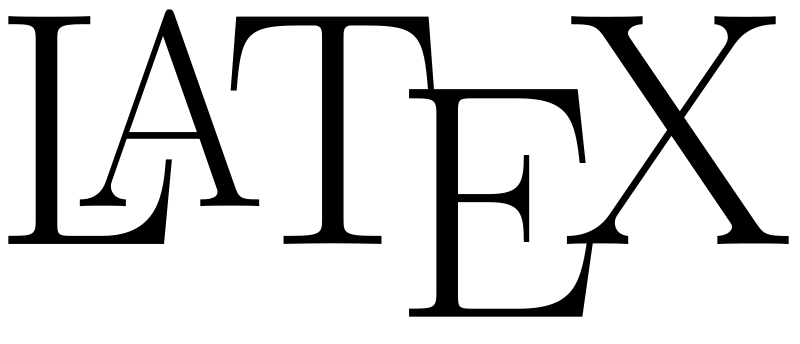
\includegraphics[width=0.80\textwidth]{figuras/latex.png}
\caption{Nome da Figura}
\label{figura1}
\end{figure}
\pagebreak
s




%capítulo 3 - Estudo de Viabilidade do Projeto proposto
\chapter{ESTUDO DE VIABILIDADE} \label{estudo}

Neste capítulo pretende-se mostrar por que o \textit{software} proposto será viável para áreas comerciais de qualquer ramo. As próximas seções falam sobre o mercado potencial, os benefícios, as oportunidades, as forças, as fraquezas, as ameaças e os concorrentes diferenciais.

\section{Mercado potencial}

\section{Benefícios}

\section{Oportunidades}

\section{Forças}

\section{Fraquezas}


\section{Ameaças}


\section{Concorrentes Diferenciais}



%capítulo 4 - Descrição do Projeto
\chapter{DESCRIÇÃO DO PROJETO} \label{capitulo}

\section{Arquitetura}

\section{Descrição do Problema}

\section{Levantamento de Requisitos}

\subsection{Requisitos Funcionais e Não Funcionais}

As tabelas \ref{rf1} a seguir, apresentam um dos requisitos levantados para o sistema.

\begin{table}[htbp!]
\caption{nome da tabela}
\begin{center}
  \begin{tabularx}{\textwidth}{|c|X|c|c|c|}
      \hline
%multicolumn é a mesclagem da linha
      \multicolumn{4}{|l|}{\textbf{RF1: requisito}} & \multicolumn{1}{l|}{\textbf{Oculto:}}\\
      \hline
      \multicolumn{5}{|p{14cm}|}{\textbf{Descrição:} a descrição}\\
      \hline
      \multicolumn{5}{|c|}{\textbf{Requisitos não funcionais}}\\
      \hline
      \textbf{Nome} & \multicolumn{1}{c|}{\textbf{Restrição}} & \textbf{Categoria} & \textbf{Desejável} & \textbf{Permanente}\\
      \hline
      \textbf{NF 1.1} & requisito. &           & ( ) & (x)\\
      \hline
    \end{tabularx}
  \end{center}
  \label{rf1}
\end{table}


\subsection{Regras de Negócio}

\begin{table}[htbp!]
  \caption{Regras de Negócio}
  \centering
      \begin{tabularx}{\textwidth}{|l|X|X|}
    \hline
      \textbf{Regra} & \textbf{Nome} & \textbf{Descrição}\\
      \hline
      RN1 & Regra & Descrição.\\
      \hline
      RN2 & Regra & Descrição.\\
      \hline
      RN3 & Regra & Descrição.\\
      \hline
      RN4 & Regra & Descrição.\\
      \hline
      RN5 & Regra & Descrição.\\
      \hline
      RN6 & Regra & Descrição.\\
      \hline 
      \end{tabularx}
  \label{regra}
\end{table}


\subsection{Descrição dos Atores}


\section{Casos de Uso}


\subsection{Diagrama de Casos de Uso}


\subsection{Descrição dos Casos de Uso}

Modelo de tabela de descrição de um caso de uso.

\begin{table}[htpb!]
 \caption{Caso de Uso: Consultar Cliente}
  \begin{center}
    \begin{tabularx}{1.0\textwidth}{|X|}
    \hline
      \textbf{CSU1:} Consultar Cliente\\
      Este caso de uso descreve as funcionalidades para consultar um cliente no sistema.\\
      \hline
      \textbf{Atores:} Funcionário, Gerente\\
      \hline
      \textbf{Pré-Condição:} O usuário deverá estar logado no sistema.\\
      \hline
      \textbf{Pós-condição:} Não possui.\\
      \hline
      \textbf{Fluxo Principal:}
      \begin{enumerate}
        \item O caso de uso inicia quando o ator clicar na página consultar cliente.
        \item O sistema apresenta o botão Consultar para ser selecionado.
        \item O Ator clica no botão Consultar.
        \item O sistema realiza a busca dos dados informados na base de dados, retorna uma mensagem e então o caso de uso se encerra.
        \item Este caso de uso se encerra.
      \end{enumerate}\\
    \hline
      \textbf{Fluxo Alternativo (A1)}
      \begin{enumerate}
      \renewcommand{\labelenumi}{\alph{enumi}.}
        \item Se na etapa 2 do fluxo principal o ator informar que não deseja mais consultar um cliente,o passo seguinte é clicar no botão Cancelar e voltará para o passo nº 2, aguardando resposta do ator.
      \end{enumerate}\\
      \hline
      \textbf{Fluxo de Exceção (E1)}
      \begin{enumerate}
      \renewcommand{\labelenumi}{\alph{enumi}.}
        \item Dados não encontrados: na etapa 3 do CASO\#01 do fluxo principal, o sistema busca os clientes, informa mensagem de erro se não encontrar e posiciona o cursor do mouse no campo com erro.
      \end{enumerate}\\
    \hline
    \end{tabularx}
  \end{center}
  \label{dcu1}
\end{table}
\pagebreak


\section{Especificação da Análise}
\subsection{Diagrama de Pacotes}

\subsection{Diagrama de Classe}

\subsection{Diagrama de Entidade e Relacionamento}

\subsection{Dicionário de Dados}

Modelo de tabela de dicionário de dados.

%% ======================================Classe Funcionario=======================================================
\begin{table}[htp!]
\caption{Classe Funcionário}
\centering
\begin{tabularx}{\textwidth}{|X|X|X|}
\hline
\multicolumn{3}{|c|}{\textbf{Classe Funcionario}} \\
 \hline 
 \multicolumn{3}{|c|}{Contém as informações do funcionário} \\
 \hline
 \textbf{ATRIBUTO} & \textbf{TIPO} & \textbf{DESCRIÇÃO} \\
 \hline
 Id\_Cliente & Int & Identifica o funcionário \\
 \hline
 CPF & String & CPF do funcionário \\
 \hline
 Nm\_Funcionario & String & Nome do funcionário \\
 \hline
 Dt\_Nascimento & String & Data de nascimento do funcionário \\
 \hline
 Sexo & String & Sexo do funcionário \\
 \hline
 Cargo & String & Cargo do funcionário \\
 \hline
 Email & String & Email pessoal do funcionário \\
 \hline
 Nr\_Tel\_Cel & String & Número celular do funcionário \\
 \hline
 Nr\_Tel\_Res & String & Número residencial do funcionário \\
 \hline
 Usuario & Usuario & Usuário do funcionário \\
 \hline
 Endereco & Endereco & Endereço do funcionário \\
\hline
\end{tabularx}{}
\end{table}

\subsection{Diagrama de Atividades}

\subsection{Diagrama de Sequência}

\section{Descrição da implementação}




%capítulo 5 - Telas do protótipo pronto (TCC2)
\chapter{TELAS DO PROTÓTIPO} \label{telas}

Neste capítulo são apresentadas as telas do protótipo.



%capítulo 6 - Validação do projeto
\chapter{VALIDAÇÃO E VERIFICAÇÃO} \label{val}

%capítulo 7 - Conclusão
\chapter{CONCLUSÃO}\label{conc}

\section{Considerações Finais}

\section{Dificuldades}

\section{Trabalhos Futuros}




%==============================================================================
%				  BIBLIOGRAFIA / REFERÊNCIAS
%==============================================================================
%Bibliografia com geração automática

%bibliografia é o nome do arquivo de bibliografia (bibliografia.bib)
\bibliography{bibliografia}{}

%abnt-alf = forma de apresentação da referência dentro do texto.
\bibliographystyle{abnt-alf}
%==============================================================================

%Bibliografia manual

\begin{thebibliography}{widest entry}
\bibitem[01]{wang} WANGENHEIM, Christiane Gresse Von; WANGENHEIM, Aldo Von. "Raciocínio Baseado em Casos", Curitiba, Atlas, 2003.
\bibitem[02]{Io02} Insercure org. \emph{The Network Explotation Tool and Security Scanner}. 2002. URL:\verb+http://www.insecure.org/nmap.+ Last Visited: 22/07/2002.
\end{thebibliography}




%==============================================================================
%				  ANEXOS (OPCIONAL)
%==============================================================================

\anexo

%Exemplo de capítulo que deve ser coloca em anexo
\chapter*{CÓDIGOS DESENVOLVIDOS}

Aqui você coloca os códigos desenvolvidos na criação do protótipo.
Um forma de inserir códigos de programação dentro do texto é:

\begin{lstlisting}
        #include 
        using namespace std;
 
        int main(int argc, char *argv[])
        {
            cout << "Ola mundo LaTeX" << endl;
        }
\end{lstlisting}

Outra possibilidade muito útil, é a importação do arquivo com o código fonte. Desta forma, se você modificar o código fonte, para atualizar o seu documento basta recompilar o arquivo LaTeX. O comando para importar código fonte para LaTeX é o seguinte:

\lstinputlisting{codigos/ola_mundo_latex.cpp}

Mais informações sobre esse assunto, entre no site: \verb+http://www.borges-solutions.com+
\verb+/inserindo-codigos-fonte-em-arquivos-latex/+



%Fim do documento
\end{document}